\documentclass[border=10pt,varwidth]{standalone}
\usepackage{tikz,tikz-3dplot}
\usetikzlibrary{angles}
\begin{document}
% ----- First plot    


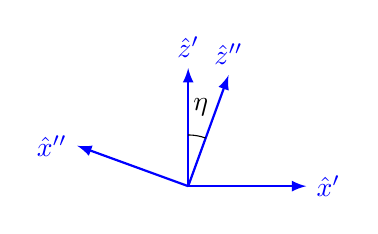
\begin{tikzpicture} [axis/.style={->,>=latex,blue,thick}]
        \coordinate (O) at (0,0);
        \def\angle{-20};
        \draw[axis] (O) -- (1.5,0) node[anchor=west]{$\hat{x}'$};
        \draw[axis] (O) -- (0,1.5) node[anchor=south]{$\hat{z}'$} coordinate(z1);
        \draw[axis,rotate=\angle] (O) -- (-1.5,0) node[anchor=east]{$\hat{x}''$};
        \draw[axis,rotate=\angle] (O) -- (0,1.5) node[anchor=south]{$\hat{z}''$} coordinate(z2);
        \pic [draw,angle radius=.65cm] {angle = z2--O--z1}; \node at (.16,1) {$\eta$};
\end{tikzpicture}


\end{document}